\documentclass{article}
\usepackage{graphicx,fancyhdr,amsmath,amssymb,amsthm,subfig,url,hyperref}
\usepackage[margin=1in]{geometry}
\usepackage{enumerate}
\usepackage{algorithm}
\usepackage{algpseudocode}
\usepackage{pifont}
 \usepackage{color}


\usepackage{tikz}
\usepackage{tabularx}
\usetikzlibrary{shapes.geometric}
\usetikzlibrary{arrows}

\renewcommand{\algorithmicrequire}{\textbf{input:}}

%----------------------- Macros and Definitions --------------------------

%%% FILL THIS OUT
\newcommand{\studentname}{Nico Chaves, Junjie (Jason) Zhu}
\newcommand{\suid}{jjzhu}
\newcommand{\exerciseset}{}
%%% END
\renewcommand{\theenumi}{\bf \Alph{enumi}}

%\theoremstyle{plain}
%\newtheorem{theorem}{Theorem}
%\newtheorem{lemma}[theorem]{Lemma}

\fancypagestyle{plain}{}
\pagestyle{fancy}
\fancyhf{}
\fancyhead[RO,LE]{\sffamily\bfseries\large  MS\&E 310 Final Project, Stanford University}
\fancyhead[LO,RE]{\sffamily\bfseries\large Multi-Block ADMM for LP}
% \fancyfoot[LO,RE]{\sffamily\bfseries\large \studentname: \suid @stanford.edu}
\fancyfoot[RO,LE]{\sffamily\bfseries\thepage}
\renewcommand{\headrulewidth}{1pt}
\renewcommand{\footrulewidth}{1pt}

\graphicspath{{figures/}}

%-------------------------------- Title ----------------------------------

\title{Multi-block ADMM Methods for Linear Programming }
\author{\studentname}

%--------------------------------- Text ----------------------------------

\begin{document}
\maketitle
\vspace{0.1in}
\maketitle



%%%%%%
\section{Introduction}
The alternating direction method of multipliers (ADMM) is a first-order method that can be used to solve various optimization problems. It splits the original problem into smaller pieces that are easier to handle during each iterative update. ADMM relies on the idea of the augmented Lagrangian method to robustify the problem and the splitting procedure makes it a proximal method that can be adopted in a wide range of optimization problems.
\newline
\newline
The goal of this project is to use ADMM to solve the primal linear programming  (LP) problem:
\begin{align}
\text{minimize}_{\mathbf{x}} &\quad \mathbf{c}^T\mathbf{x} \tag{OPT1}\label{OPT1} \\
\text{subject to } &\quad  A \mathbf{x} = \mathbf{b},  \nonumber \\
&\quad \mathbf{x} \geq \mathbf{0} \nonumber 
\end{align}
or its dual
\begin{align}
\text{maximize}_{\mathbf{y}, \mathbf{s}} &\quad \mathbf{b}^T\mathbf{y}  \tag{OPT2}\label{OPT2} \\
\text{subject to } &\quad  A^T \mathbf{y}  + \mathbf{s} = \mathbf{c},  \nonumber \\
&\quad \mathbf{s} \geq \mathbf{0} \nonumber.
\end{align}
In this report, we first re-formulate the problems to derive closed form updates for the primal and the dual LP problems. We then approach each problem using the corresponding interior-point method. For each of these four approaches, we are specifically interested in the effect of preconditioning and block-splitting on the convergence rate and the accuracy of the solvers. We implemented all of the algorithms in MATLAB and ran experiments to test how these methods perform on different simulated problems.

%%%%%%%%%%
\vspace{0.1in}
\subsection*{Preconditioning}
In this report, we demonstrate the effect of preconditioning on the various ADMM approaches mentioned above. To precondition a linear programming problem, one first computes 
\begin{align}
A' = (AA^T )^{-1/2}A , \quad \quad \mathbf{b}' =(AA^T )^{-1/2}\mathbf{b},
\end{align}
and then substitutes $A'$ and $\mathbf{b}'$ for $A$ and $\mathbf{b}$ in the original problems \eqref{OPT1} and \eqref{OPT2}. Clearly, this re-formulation does not change the feasible regions for  \eqref{OPT1} or \eqref{OPT2}. 

%%%%%%%%%%
\vspace{0.1in}
%%%%%%%%%%
\vspace{0.1in}
\subsection*{Block-Splitting ADMM}
As we will show in Section 2, ADMM requires computation of a potentially large matrix inverse. Since matrix inversion is approximately cubic in complexity, this computation may become the bottleneck for sufficiently large problems. By splitting the decision variables into blocks and updating the blocks sequentially, one can reduce the runtime by computing multiple small matrix inverses instead of a single large matrix inverse.

In this report, we demonstrate the effect of block splitting on ADMM. We demonstrate that block splitting with 3 or more blocks may not converge to the optimal solution. However, we demonstrate through experiments that randomly permuting the update order of the blocks at each iteration resolves this issue.

We also demonstrate that block splitting and preconditioning work well when used together. However, the preconditioning approach we consider in this report requires a matrix inverse computation. Therefore, one still may suffer from a slow matrix inversion if one uses preconditioning. In our future work, we plan to study inverse-free preconditioning methods such as Cholesky preconditioning.

%%%%%%%%%%
\vspace{0.5in}
\section{Basic ADMM for LP}
\vspace{0.1in}
\subsection*{Primal Re-formulation}
We re-formulate the primal LP problem as:
\begin{align}
\text{minimize}_{ \mathbf{x}_{1}, \mathbf{x}_{2}} &\quad \mathbf{c}^T\mathbf{x}_1 \tag{OPT3}\label{OPT3} \\
\text{subject to  \ \  } &\quad  A \mathbf{x}_{1} = \mathbf{b}  \nonumber \\
&\quad \mathbf{x}_{1}  - \mathbf{x}_{2} = \mathbf{0}  \nonumber \\
&\quad \mathbf{x}_{2} \geq \mathbf{0} \nonumber 
\end{align}
and consider the split Lagrangian function:
\[
L^{P}(\mathbf{x}_{1},\mathbf{x}_{2},\mathbf{y} ,\mathbf{s})=\mathbf{c}^{T}\mathbf{x}_{1}-\mathbf{y}^{T}\left(A\mathbf{x}_{1}-\mathbf{b}\right)-\mathbf{s}^{T}\left(\mathbf{x}_{1}-\mathbf{x}_{2}\right)+\frac{\beta}{2}\left(\left\Vert A\mathbf{x}_{1}-\mathbf{b}\right\Vert ^{2}+\left\Vert \mathbf{x}_{1}-\mathbf{x}_{2}\right\Vert ^{2}\right).
\]
\subsection*{Primal Update}
To obtain the updates for the primal variables in ADMM, we must compute the gradient of these variables and set the gradient to zero. Here we update $\mathbf{x}_{1}$ and $\mathbf{x}_{2}$ sequentially using the update function for each respectively:
\begin{align}
\mathbf{x}_{1}^{k+1} & = \arg \min_{\mathbf{x}_{1}^{k}} L^{P}(\mathbf{x}_{1}^{k},\mathbf{x}_{2}^{k},\mathbf{y}^{k},\mathbf{s}^k),\\
\mathbf{x}_{2}^{k+1} & = \arg \min_{\mathbf{x}_{2}^{k} \geq 0} L^{P}(\mathbf{x}_{1}^{k+1},\mathbf{x}_{2}^{k},\mathbf{y}^{k},\mathbf{s}^k).
\end{align}
To solve for $\mathbf{x}_{1}$, we set the gradient to zero:
\[
\nabla_{\mathbf{x}_{1}}L^{P}(\mathbf{x}_{1},\mathbf{x}_{2},\mathbf{y}, \mathbf{s})=\mathbf{c}-A^{T}\mathbf{y}-\mathbf{s}+\beta\left(A^{T}\left(A\mathbf{x}_{1}-\mathbf{b}\right)+\left(\mathbf{x}_{1}-\mathbf{x}_{2}\right)\right) = \mathbf{0}
\]
and we obtain the update step for $\mathbf{x}_{1}$:
\begin{align}\label{eq:x1_primal_update}
\mathbf{x}_{1}^{k+1} = \left(A^{T}A+I\right)^{-1}\left(\frac{1}{\beta}A^{T}\mathbf{y}^k+\frac{1}{\beta}\mathbf{s}^k-\frac{1}{\beta}\mathbf{c}+A^{T}\mathbf{b}^k+\mathbf{x}_{2}^k\right)
\end{align}
Similarly, we solve
\[
\nabla_{\mathbf{x}_{2}}L^{P}=\mathbf{s}+\beta\left(\mathbf{x}_{2}-\mathbf{x}_{1}\right) = \mathbf{0}
\]
to obtain the update for $\mathbf{x}_{2}$. Since the elements of $\mathbf{x}_{2}$ are separable, we can update each one independently as follows:
\begin{align}
{x}_{2,j}^{k+1} = \max\left\{ {x}_{1,j}^k-\frac{1}{\beta}{s}_j^k,0\right\} \text{ for $j = 1,..,n$}.
\end{align}
Next, we update the multipliers $\mathbf{y}$ and $\mathbf{s}$ using
\begin{align}\label{eq:y_primal_update}
\mathbf{y}^{k+1} &= \mathbf{y}^{k} + \beta (A \mathbf{x}_1^{k+1}  - \mathbf{b}) 
\end{align}
\begin{align}\label{eq:s_primal_update}
\mathbf{s}^{k+1} &= \mathbf{s}^{k}  - \beta  (\mathbf{x}_1^{k+1}  -\mathbf{x}_2^{k+1} )
\end{align}
These two updates guarantee that $\left(\mathbf{x}_1^{k+1}, \mathbf{x}_2^{k+1}, \mathbf{y}^{k+1}, \mathbf{s}^{k+1}\right)$ is dual feasible, i.e.,
\begin{align*}
\nabla_{\mathbf{x}_{1}, \mathbf{x}_{2}}L^{P}(\mathbf{x}_{1}^k,\mathbf{x}_{2}^k,\mathbf{y}^k ,\mathbf{s}^k)=\mathbf{0}.
\end{align*}
We terminate when the solution is primal feasible, i.e., $A \mathbf{x}_1^{k+1}  - \mathbf{b} \approx \mathbf{0}$ and $\mathbf{x}_1^{k+1}  -\mathbf{x}_2^{k+1} \approx \mathbf{0}$.

%%%%%%%%%%
\vspace{0.1in}
\subsection*{Dual Re-formulation}
We convert the problem of the dual to a minimization problem to apply ADMM:
\begin{align}
\text{minimize}_{\mathbf{y}, \mathbf{s}} &\quad -\mathbf{b}^T\mathbf{y}  \tag{OPT4}\label{OPT4} \\
\text{subject to } &\quad  A^T \mathbf{y}  + \mathbf{s} = \mathbf{c},  \nonumber \\
&\quad \mathbf{s} \geq \mathbf{0} \nonumber.
\end{align}
The dual LP problem does not require additional re-formulation because the non-zero variable $\mathbf{s}$ is already separable, which can be observed via the dual Lagrangian function:
\[
L^{d}(\mathbf{y},\mathbf{s},\mathbf{x})=-\mathbf{b}^{T}\mathbf{y}-\mathbf{x}^{T}\left(A^{T}\mathbf{y}+\mathbf{s}-\mathbf{c}\right)+\frac{\beta}{2}\left\Vert A^{T}\mathbf{y}+\mathbf{s}-\mathbf{c}\right\Vert ^{2}.
\]
Note that $\mathbf{x}$ would be non-positive since we changed maximization to minimization and we would need to take the negative of $\mathbf{x}$ of the final solution as the solution to the original LP.

%%%%%%%%%%
\vspace{0.1in}
\subsection*{Dual Update}
Similar to the primal updates, we use the updates for the primal variables $\mathbf{y}$ and $\mathbf{s}$ according to 
\begin{align}
\mathbf{y}^{k+1} & = \arg \min_{\mathbf{y}} L^{d}(\mathbf{y}^{k},\mathbf{s}^k, \mathbf{x}^{k}),\\
\mathbf{s}^{k+1} & = \arg \min_{\mathbf{s} \geq 0} L^{d}(\mathbf{y}^{k+1},\mathbf{s}^k,\mathbf{x}^{k}).
\end{align}
Setting the gradients with respect to $\mathbf{y}$ and $\mathbf{s}$ to zero, i.e.,
\begin{align}
\nabla_{\mathbf{y}}L^{d}(\mathbf{y},\mathbf{s},\mathbf{x}) & =  -\mathbf{b}-A\mathbf{x}+\beta A\left(A^{T}\mathbf{y}+\mathbf{s}-\mathbf{c}\right)  = \mathbf{0}, \label{eq:dual_y} \\
\nabla_{\mathbf{s}}L^{d}(\mathbf{y},\mathbf{s},\mathbf{x}) & =  -\mathbf{x}+\beta\left(A^{T}\mathbf{y}+\mathbf{s}-\mathbf{c}\right) =  \mathbf{0},
\end{align}
we have the updates for $\mathbf{y}$ (least-squares problem) and $\mathbf{s}$:
\begin{align}\label{eq:y_dual_update}
\mathbf{y}^{k+1} = \left(AA^{T}\right)^{-1}\left(\frac{1}{\beta}\left(A\mathbf{x}^{k}+\mathbf{b}\right)-A\mathbf{s}^{k}+A\mathbf{c}\right),
\end{align}
\begin{align}\label{eq:s_dual_update}
s_j^{k+1} = \max\left\{ \frac{1}{\beta}{x}_j^k-(A^{T}\mathbf{y}^{k+1})_j+{c}_j,0\right\}.
\end{align}
We can update the multipliers $\mathbf{x}$ by
\begin{align}\label{eq:x_dual_update}
\mathbf{x}^{k+1} = \mathbf{x}^k - \beta\left(A^T \mathbf{y}^{k+1} + \mathbf{s}^{k+1} - \mathbf{c}\right).
\end{align}
We terminate and declare optimality when $A \mathbf{x}^{k+1} + \mathbf{b} \approx \mathbf{0}$.


%%%%%%%%%%%%%%%%%%%%%%%%%%%%
\vspace{0.5in}
\section{Interior-Point ADMM for LP}

\vspace{0.1in}
\subsection*{Primal LP Updates}
We can use the previous formulation in \eqref{OPT3} with  $\mathbf{x}_{1}$ and $\mathbf{x}_{2}$ using the log barrier function:
\begin{align}
\text{minimize}_{ \mathbf{x}_{1}, \mathbf{x}_{2}} &\quad \mathbf{c}^T\mathbf{x}_1 + \mu \sum_j \ln( {x}_{2,j} )\tag{OPT5}\label{OPT5} \\
\text{subject to  \ \  } &\quad  A \mathbf{x}_{1} = \mathbf{b},  \nonumber \\
&\quad \mathbf{x}_{1}  - \mathbf{x}_{2} = \mathbf{0}, \nonumber \\
&\quad \mathbf{x}_{2} > \mathbf{0}, \nonumber 
\end{align}
where the Lagrangian function is given by
\[
L_{\mu}^{p}(\mathbf{x}_{1},\mathbf{x}_{2},\mathbf{y}, \mathbf{s})=\mathbf{c}^{T}\mathbf{x}_{1}-\mu\sum_{j}\ln\left(x_{2,j}\right)-\mathbf{y}^{T}\left(A\mathbf{x}_{1}-\mathbf{b}\right)-\mathbf{s}^{T}\left(\mathbf{x}_{1}-\mathbf{x}_{2}\right)+\frac{\beta}{2}\left(\left\Vert A\mathbf{x}_{1}-\mathbf{b}\right\Vert ^{2}+\left\Vert \mathbf{x}_{1}-\mathbf{x}_{2}\right\Vert ^{2}\right).
\]
Setting the gradient of this to zero yields the same update for $\mathbf{x}_1$ as in \eqref{eq:x1_primal_update}.
However, the we need to modify the update for $\mathbf{x}_2$ as now we have:
\begin{align}
s_j - \frac{\mu}{x_{2,j}} + \beta(x_{2,j} - x_{1,j}) = 0
\end{align}
which yields 
\begin{align}
x_{2,j} = \frac{1}{2\beta}\left(\beta x_{1,j} - s_j  + \sqrt{\beta^2 x_{1,j}^2 - 2\beta s_j x_{1,j} + s_j^2 + 4\beta\mu } \right), \text{ for $j = 1,..,n$}
\end{align}
The update equations for $\mathbf{y}$ and $\mathbf{s}$ remain the same as in \eqref{eq:y_primal_update} and \eqref{eq:s_primal_update}. 
The update equation for $\mathbf{x}$ remains the same as in \eqref{eq:x_dual_update}. At the end of each iteration, we update $\mu^{k+1} = \gamma \mu^k$ for some constant $\gamma<1$, and the terminal condition remains the same as the non-interior-point method. 

\vspace{0.1in}
\subsection*{Dual LP Updates}
We can use the previous formulation in \eqref{OPT4} using the barrier function:
\begin{align}
\text{minmize}_{\mathbf{y}, \mathbf{s}} &\quad -\mathbf{b}^T\mathbf{y} + \mu \sum_j \ln (s_j)  \tag{OPT6}\label{OPT6} \\
\text{subject to } &\quad  A^T \mathbf{y}  + \mathbf{s} = \mathbf{c},  \nonumber \\
&\quad \mathbf{s} > \mathbf{0} \nonumber.
\end{align}
where the Lagrangian function is given by
\[
L_{\mu}^{d}(\mathbf{y},\mathbf{s},\mathbf{x})=-\mathbf{b}^{T}\mathbf{y}-\mu\sum_{j}\ln\left(s_{j}\right)-\mathbf{x}^{T}\left(A^{T}\mathbf{y}+\mathbf{s}-\mathbf{c}\right)+\frac{\beta}{2}\left\Vert A^{T}\mathbf{y}+\mathbf{s}-\mathbf{c}\right\Vert ^{2}.
\]
Setting the gradient of this to zero yields the same update for $\mathbf{y}$ as in \eqref{eq:y_dual_update} 
However, the we need to modify the update for $\mathbf{s}$ as now we have:
\begin{align}
- \frac{\mu}{s_j} + x_j  + \beta \left(s_j - (\mathbf{c} - (A^T \mathbf{y}))_j\right)= 0
\end{align}
which yields 
\begin{align}
s_j = \frac{1}{2\beta}\left(\beta (\mathbf{c} - (A^T \mathbf{y}))_j + x_j  + \sqrt{\beta^2 (\mathbf{c} - (A^T \mathbf{y}))_j^2 - 2\beta (\mathbf{c} - (A^T \mathbf{y}))_j x_{j} + x_j^2 + 4\beta\mu } \right), \text{ for $j = 1,..,n$}
\end{align}
The update equation for $\mathbf{x}$ remain the same as in \eqref{eq:x_dual_update}. At the end of each iteration, we update $\mu^{k+1} = \gamma \mu^k$ for some constant $\gamma<1$, and the terminal condition remains the same as the non-interior-point method.



%%%%%%%%%%
\vspace{0.5in}
\section{Multi-Block ADMM}

As mentioned previously, splitting the problem into blocks may reduce computation time by avoiding a large matrix inversion.
However, when the set of variables are separable, it may not be necessary to apply block updates on them because at the end of each iteration, these separable variables would take identical values no matter how they are grouped. For separable variables, the most efficient way would be updating each variable separately (or in parallel). Thus, we only need to consider the cases where we split $\mathbf{x_1}$ in the primal problems (i.e.,  \eqref{OPT3} and \eqref{OPT5}), or to split $\mathbf{y}$ in the primal problems (i.e.,  \eqref{OPT4} and \eqref{OPT6}).

\subsection*{Primal with Block Splitting (B=2 Blocks)}

To help make our derivations concrete, we first consider splitting the problem into $B=2$ blocks of equal size as follows:
\[
\mathbf{x}_{1}=\begin{bmatrix}\mathbf{x}_{1,1}\\
\mathbf{x}_{1,2}
\end{bmatrix},
 \ \  
A=\begin{bmatrix}A_{1} & A_{2}\end{bmatrix},
\ \ 
\mathbf{c}=\begin{bmatrix}\mathbf{c}_{1}\\
\mathbf{c}_{2}
\end{bmatrix}
\]
Then the Lagrangian can be expressed as:
\begin{eqnarray*}
L^{P}(\mathbf{x}_{1},\mathbf{x}_{2},\mathbf{y}) & = & \mathbf{c}_{1}^{T}\mathbf{x}_{1,1}+\mathbf{c}_{2}^{T}\mathbf{x}_{1,2}-\mathbf{y}^{T}\left(A_{1}\mathbf{x}_{1,1}+A_{2}\mathbf{x}_{1,2}-\mathbf{b}\right)-\mathbf{s}_{1}^{T}\left(\mathbf{x}_{1,1}-\mathbf{x}_{2,1}\right)-\mathbf{s}_{2}^{T}\left(\mathbf{x}_{1,2}-\mathbf{x}_{2,2}\right)\\
 &  & +\frac{\beta}{2}\left(\left\Vert A_{1}\mathbf{x}_{1,1}+A_{2}\mathbf{x}_{1,2}-\mathbf{b}\right\Vert ^{2}+\left\Vert \mathbf{x}_{1,1}-\mathbf{x}_{2,1}\right\Vert ^{2}+\left\Vert \mathbf{x}_{1,2}-\mathbf{x}_{2,2}\right\Vert ^{2}\right)
\end{eqnarray*}
Taking the gradient with respect to the 1st block of $\mathbf{x}_{1}$:
\[
\nabla_{\mathbf{x}_{1,1}}L^{P}(\mathbf{x}_{1},\mathbf{x}_{2},\mathbf{y})=\mathbf{c}_{1}-A_{1}^{T}\mathbf{y}-\mathbf{s}_{1}+\beta\left(A_{1}^{T}\left(A_{1}\mathbf{x}_{1,1}+A_{2}\mathbf{x}_{1,2}-\mathbf{b}\right)+\left(\mathbf{x}_{1,1}-\mathbf{x}_{2,1}\right)\right)
\]
Setting the gradient to 0, we obtain the update for $\mathbf{x}_{1,1}$:
\[
\mathbf{x}_{1,1}^{k+1}=\left(A_{1}^{T}A_{1}+I\right)^{-1}\left(\frac{1}{\beta}A_{1}^{T}\mathbf{y}+\frac{1}{\beta}\mathbf{s}_{1}-\frac{1}{\beta}\mathbf{c}_{1}+A_{1}^{T}\mathbf{b}+\mathbf{x}_{2,1}^{k}-A_{1}^{T}A_{2}\mathbf{x}_{1,2}^{k}\right)
\]
By symmetry, the update step for the 2nd block of $\mathbf{x}_{1}$
is:
\[
\mathbf{x}_{1,2}^{k+1}=\left(A_{2}^{T}A_{2}+I\right)^{-1}\left(\frac{1}{\beta}A_{2}^{T}\mathbf{y}+\frac{1}{\beta}\mathbf{s}_{2}-\frac{1}{\beta}\mathbf{c}_{2}+A_{2}^{T}\mathbf{b}+\mathbf{x}_{2,2}^{k}-A_{2}^{T}A_{1}\mathbf{x}_{1,1}^{k+1}\right)
\]
Note that here we use $\mathbf{x}_{1,1}^{k+1}$ to update $\mathbf{x}_{1,2}$. Our results show that when $B>2$ blocks, one may need to randomly permute the update order. As a result, on some iterations, we may first update $\mathbf{x}_{1,2}$, then use the new value to update $\mathbf{x}_{1,1}$. 

\subsection*{Primal Block Splitting (For a General Number of Blocks)}

We can easily extend the above result to a general number of blocks $B$. Let $U$ denote the set of blocks which have already been updated at the current iteration. To update block $i$ of $\mathbf{x}_{1}$, we compute:
\[
\mathbf{x}_{1,i}^{k+1}=\left(A_{i}^{T}A_{i}+I\right)^{-1}\left(\frac{1}{\beta}A_{i}^{T}\mathbf{y}+\frac{1}{\beta}\mathbf{s}_{i}-\frac{1}{\beta}\mathbf{c}_{i}+A_{i}^{T}\mathbf{b}+\mathbf{x}_{2,i}^{k}-\sum_{j\neq i,j\in U}A_{i}^{T}A_{j}\mathbf{x}_{1,j}^{k+1}-\sum_{j\neq i,j\notin U}A_{i}^{T}A_{j}\mathbf{x}_{1,j}^{k}\right)
\]
where $A_{i}$ refers to the $i^{\text{th}}$ block of columns of $A$.

\vspace{0.1in}
\subsection*{Dual ADMM With Block Splitting (B=2 Blocks)}
Now, we derive the corresponding update for the dual ADMM with block splitting. Again, we first consider $B=2$ case and split the problem into 2 blocks of equal size:

\[
\mathbf{y}=\begin{bmatrix}\mathbf{y}_{1}\\
\mathbf{y}_{2}
\end{bmatrix},
\ \
A^{T}=\begin{bmatrix}A_{1}^{T} & A_{2}^{T}\end{bmatrix},
\ \ 
\mathbf{b}=\begin{bmatrix}\mathbf{b}_{1}\\
\mathbf{b}_{2}
\end{bmatrix}
\]

Then the Lagrangian can be expressed as:

\[
L^{d}(\mathbf{y},\mathbf{s},\mathbf{x})=-\mathbf{b}_{1}^{T}\mathbf{y}_{1}-\mathbf{b}_{2}^{T}\mathbf{y}_{2}-\mathbf{x}^{T}\left(A_{1}^{T}\mathbf{y}_{1}+A_{2}^{T}\mathbf{y}_{2}+\mathbf{s}-\mathbf{c}\right)+\frac{\beta}{2}\left\Vert A_{1}^{T}\mathbf{y}_{1}+A_{2}^{T}\mathbf{y}_{2}+\mathbf{s}-\mathbf{c}\right\Vert ^{2}
\]


Differentiating with respect to $\mathbf{y}_{1}$:

\[
\nabla_{\mathbf{y}_{1}}L^{d}(\mathbf{y},\mathbf{s},\mathbf{x})=-\mathbf{b}_{1}-A_{1}\mathbf{x}+\beta A_{1}\left(A_{1}^{T}\mathbf{y}_{1}+A_{2}^{T}\mathbf{y}_{2}+\mathbf{s}-\mathbf{c}\right)
\]

Setting the gradient to 0, we obtain the update for $\mathbf{y}_{1}$:
\begin{eqnarray*}
A_{1}\left(A_{1}^{T}\mathbf{y}_{1}^{k+1}+A_{2}^{T}\mathbf{y}_{2}^{k}+\mathbf{s}-\mathbf{c}\right) & = & \frac{1}{\beta}\left(A_{1}\mathbf{x}+\mathbf{b}_{1}\right)\\
A_{1}A_{1}^{T}\mathbf{y}_{1}^{k+1} & = & \frac{1}{\beta}\left(A_{1}\mathbf{x}+\mathbf{b}_{1}\right)-A_{1}\left(A_{2}^{T}\mathbf{y}_{2}^{k}+\mathbf{s}-\mathbf{c}\right)\\
\mathbf{y}_{1}^{k+1} & = & \left(A_{1}A_{1}^{T}\right)^{-1}\left(\frac{1}{\beta}\left(A_{1}\mathbf{x}+\mathbf{b}_{1}\right)-A_{1}\left(A_{2}^{T}\mathbf{y}_{2}^{k}+\mathbf{s}-\mathbf{c}\right)\right)
\end{eqnarray*}


By symmetry, the update for $\mathbf{y}_{2}$ is:

\[
\mathbf{y}_{2}^{k+1}=\left(A_{2}A_{2}^{T}\right)^{-1}\left(\frac{1}{\beta}\left(A_{2}\mathbf{x}+\mathbf{b}_{2}\right)-A_{2}\left(A_{1}^{T}\mathbf{y}_{1}^{k+1}+\mathbf{s}-\mathbf{c}\right)\right)
\]


assuming that we update $\mathbf{y}_{2}$ after $\mathbf{y}_{1}$. As in the primal case, we may want to randomly permute the update order at each iteration.
\vspace{0.1in}
\subsection*{Dual Block Splitting (For a General Number of Blocks)}

We can easily extend the above result to a general number of blocks. Let $U$ denote the set of blocks which have already been updated at the current iteration. To update block $i$ of $\mathbf{y}$:
\[
\mathbf{y}_{i}^{k+1}=\left(A_{i}A_{i}^{T}\right)^{-1}\left(\frac{1}{\beta}\left(A_{i}\mathbf{x}+\mathbf{b}_{i}\right)-\sum_{j\neq i,j\in U}A_{i}A_{j}^{T}\mathbf{y}_{j}^{k+1}-\sum_{j\neq i,j\notin U}A_{i}A_{j}^{T}\mathbf{y}_{j}^{k}-A_{i}\left(\mathbf{s}-\mathbf{c}\right)\right)
\]
\vspace{0.1in}
{ \subsection*{Using Preconditioning for Dual Block Splitting}
Here, we show that block-splitting yields the same result as non-block-splitting if preconditioning is already applied to the dual problem. 

A sufficient condition for the variables to be separable is when the coefficient of these variables the gradient function is the identify matrix. Interestingly, we show that when preconditioning is applied to the dual LP problem (whether or not implemented with the interior point method), the variables $\mathbf{y}$ become separable. To see this, consider the update equation \eqref{eq:dual_y}, where the coefficient of $\mathbf{y}$ is $A A^T$. When pre-conditioning is applied, we have
\[
A' (A')^T  = (AA^T )^{-1/2}A A^T (AA^T )^{-1/2} =  (AA^T )^{-1/2}(AA^T )^{1/2} (AA^T )^{1/2} (AA^T )^{-1/2}  = I.
\]
Therefore, the variables in $\mathbf{y}$ become separable and block-splitting the same result as non-block-splitting at the end of each iteration when preconditioning is applied. 

%%%%%%%%%%%%%%%%%%%%%
\newpage
\section{Experiments and Results}

We evaluated the performance of the different ADMM approaches by randomly simulating LP problems and recording the number of iterations needed to converge. In particular, we simulated LP problems given by \eqref{OPT1} by randomly selecting $A\in\mathbb{R}^{m \times n}$ and $c\in\mathbb{R}^{n}$. We only considered feasible problems. To ensure feasibility, we randomly selected a feasible point $\mathbf{x}_{\text{feas}}\geq0$ and let $\mathbf{b}=A\mathbf{x}_{\text{feas}}$. We considered a solution to be optimal when $\left|A\mathbf{x}-\mathbf{b}\right|<10^{-3}$ (for the primal formulation) or $\left|A\mathbf{x}+\mathbf{b}\right|<10^{-3}$ (for the dual formulation). For interior point algorithms, we use $\gamma=0.99$, i.e. at each iteration, we update the parameter $\mu$ using $\mu^{k+1} = 0.99 \times \mu^k$. Each set of experiments is described in more detail below.

\subsection*{Preconditioning with No Block-Splitting}

First, we were interested in how preconditioning affects convergence rate of the basic primal and dual ADMM algorithms in \eqref{OPT3} and \eqref{OPT4}. For simplicity, we did not apply block splitting. We evaluated the two algorithms over 10 random problems of size $50 \times 300$. 

We evaluated how sensitive these ADMM LP algorithms are to the $\beta$ parameter in the augmented Lagrangian. For each algorithm, we recorded the number of iterations required to converge as a function of $\beta$. The results  are shown in Figure \ref{fig:base_p_d}. We observe that all of the ADMM approaches are relatively insensitive to $\beta$. For the rest of our experiments, we fixed $\beta=0.9$. Choosing a different value of $\beta$ should not have much effect on the rest of our results. 

Additionally, we notice that the basic primal ADMM implementation converges faster than the basic dual ADMM, but when preconditioning is applied (on the same problems), the dual converges faster whereas the primal converges slightly slower. 
\newline
\newline
\newline
\begin{figure*}[ht]
	\centering
	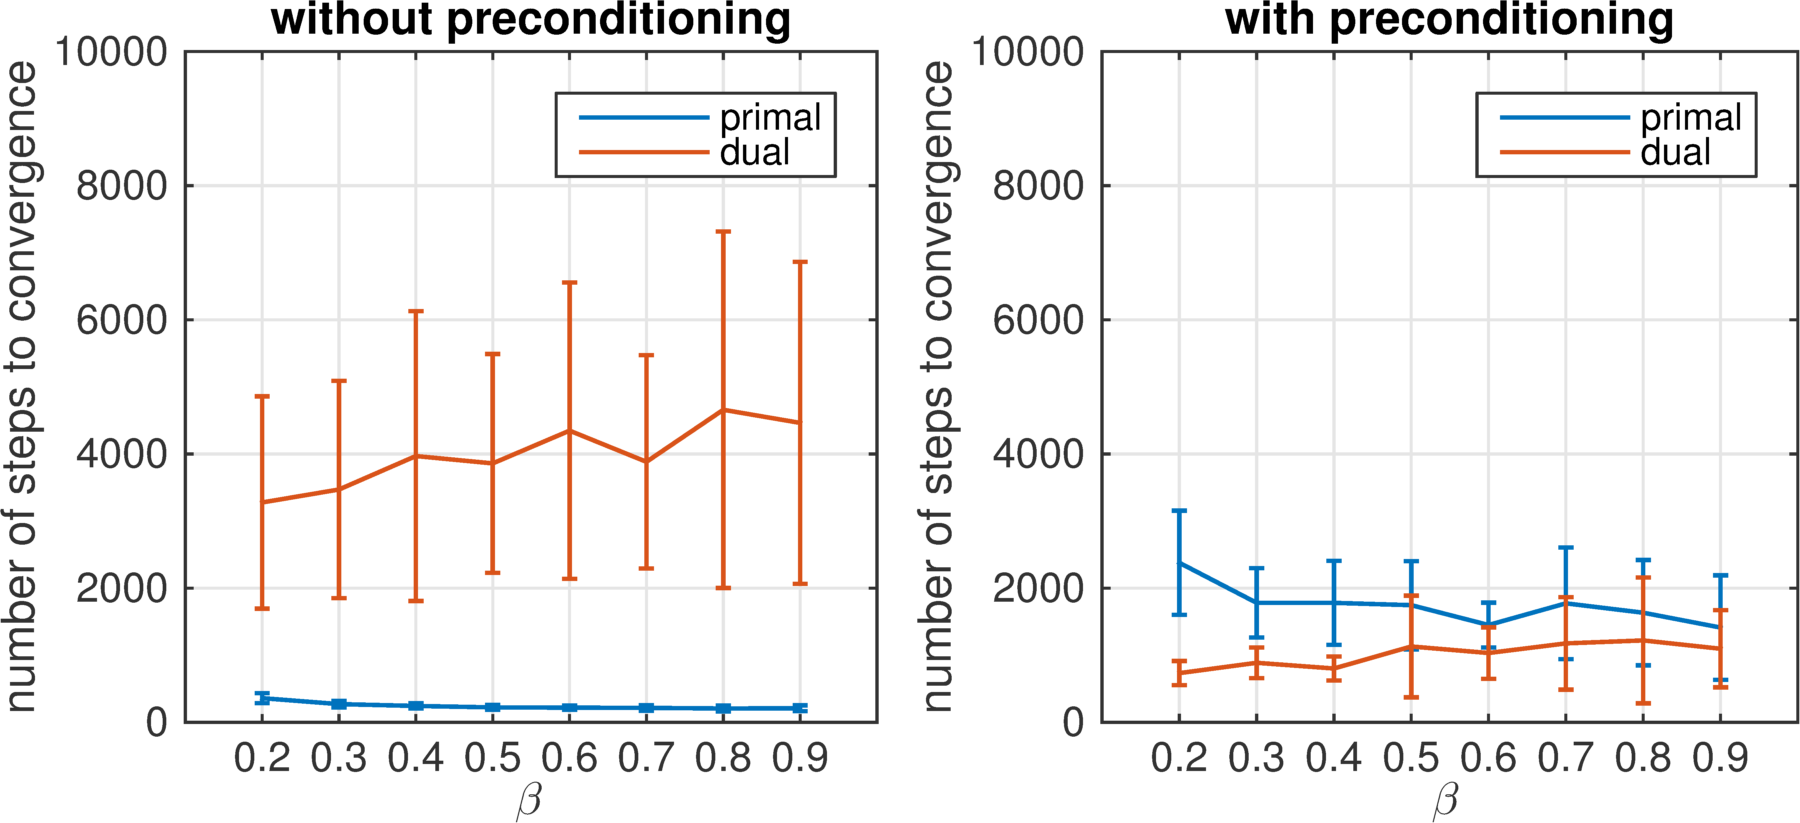
\includegraphics[width=0.8\textwidth]{../figures/primal_dual_preconditioning.png}
	\caption{Results on 10 random LP problem of size $50 \times 300$. }
	\label{fig:base_p_d}
\end{figure*}
\newpage
\subsection*{Baseline Block-splitting (No Random Permutation, No Preconditioning)}
To establish a baseline, we evaluated the ADMM solvers using sequential updating (i.e. we did not randomly permute the block update order) and without using preconditioning. The results of this experiment are shown in Figure \ref{fig:nop_nor}. In the figure, $B$ represents the number of blocks ($B=1$ indicates that no splitting was performed). Note that when $B>2$, the problem does not necessarily converge for the primal. As we will see in the following experiments, we can improve performance by introducing random permutations or preconditioning.
\newline
\newline
\newline
\newline

\begin{figure*}[h]
	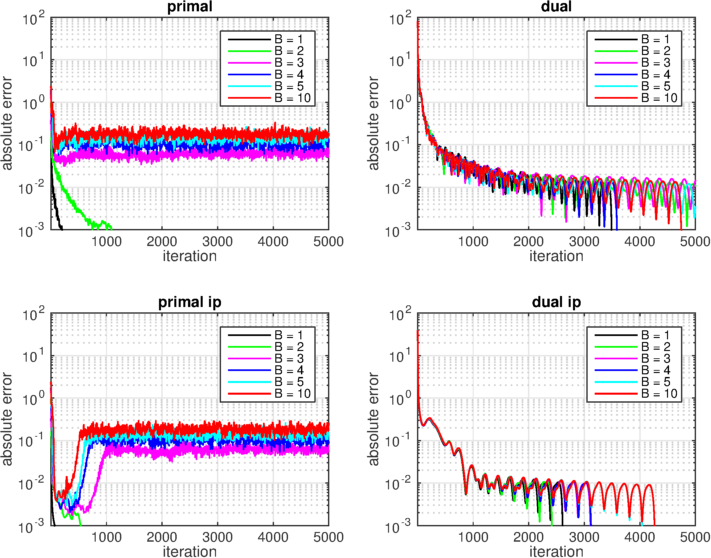
\includegraphics[width=\textwidth]{../figures/noprecond_norndperm.png}
	\caption{Results on a random LP problem of size $50 \times 300$. No preconditioning and no random permutation.}
	\label{fig:nop_nor}
\end{figure*}
\newpage
\subsection*{Block-splitting with Random Permutation (No Preconditioning)}

In this set of experiments, we randomly permuted the update order of the block variables at each iteration. The results are shown in Figure \ref{fig:nop_r}. When using random permutation, the primal now converges for all block sizes. Note that splitting the primal into more blocks requires more iterations. However, performing block splitting may still result in lower overall runtime because of the faster inverse computations. 
\newline
\newline
\newline
\newline
\begin{figure*}[h]
	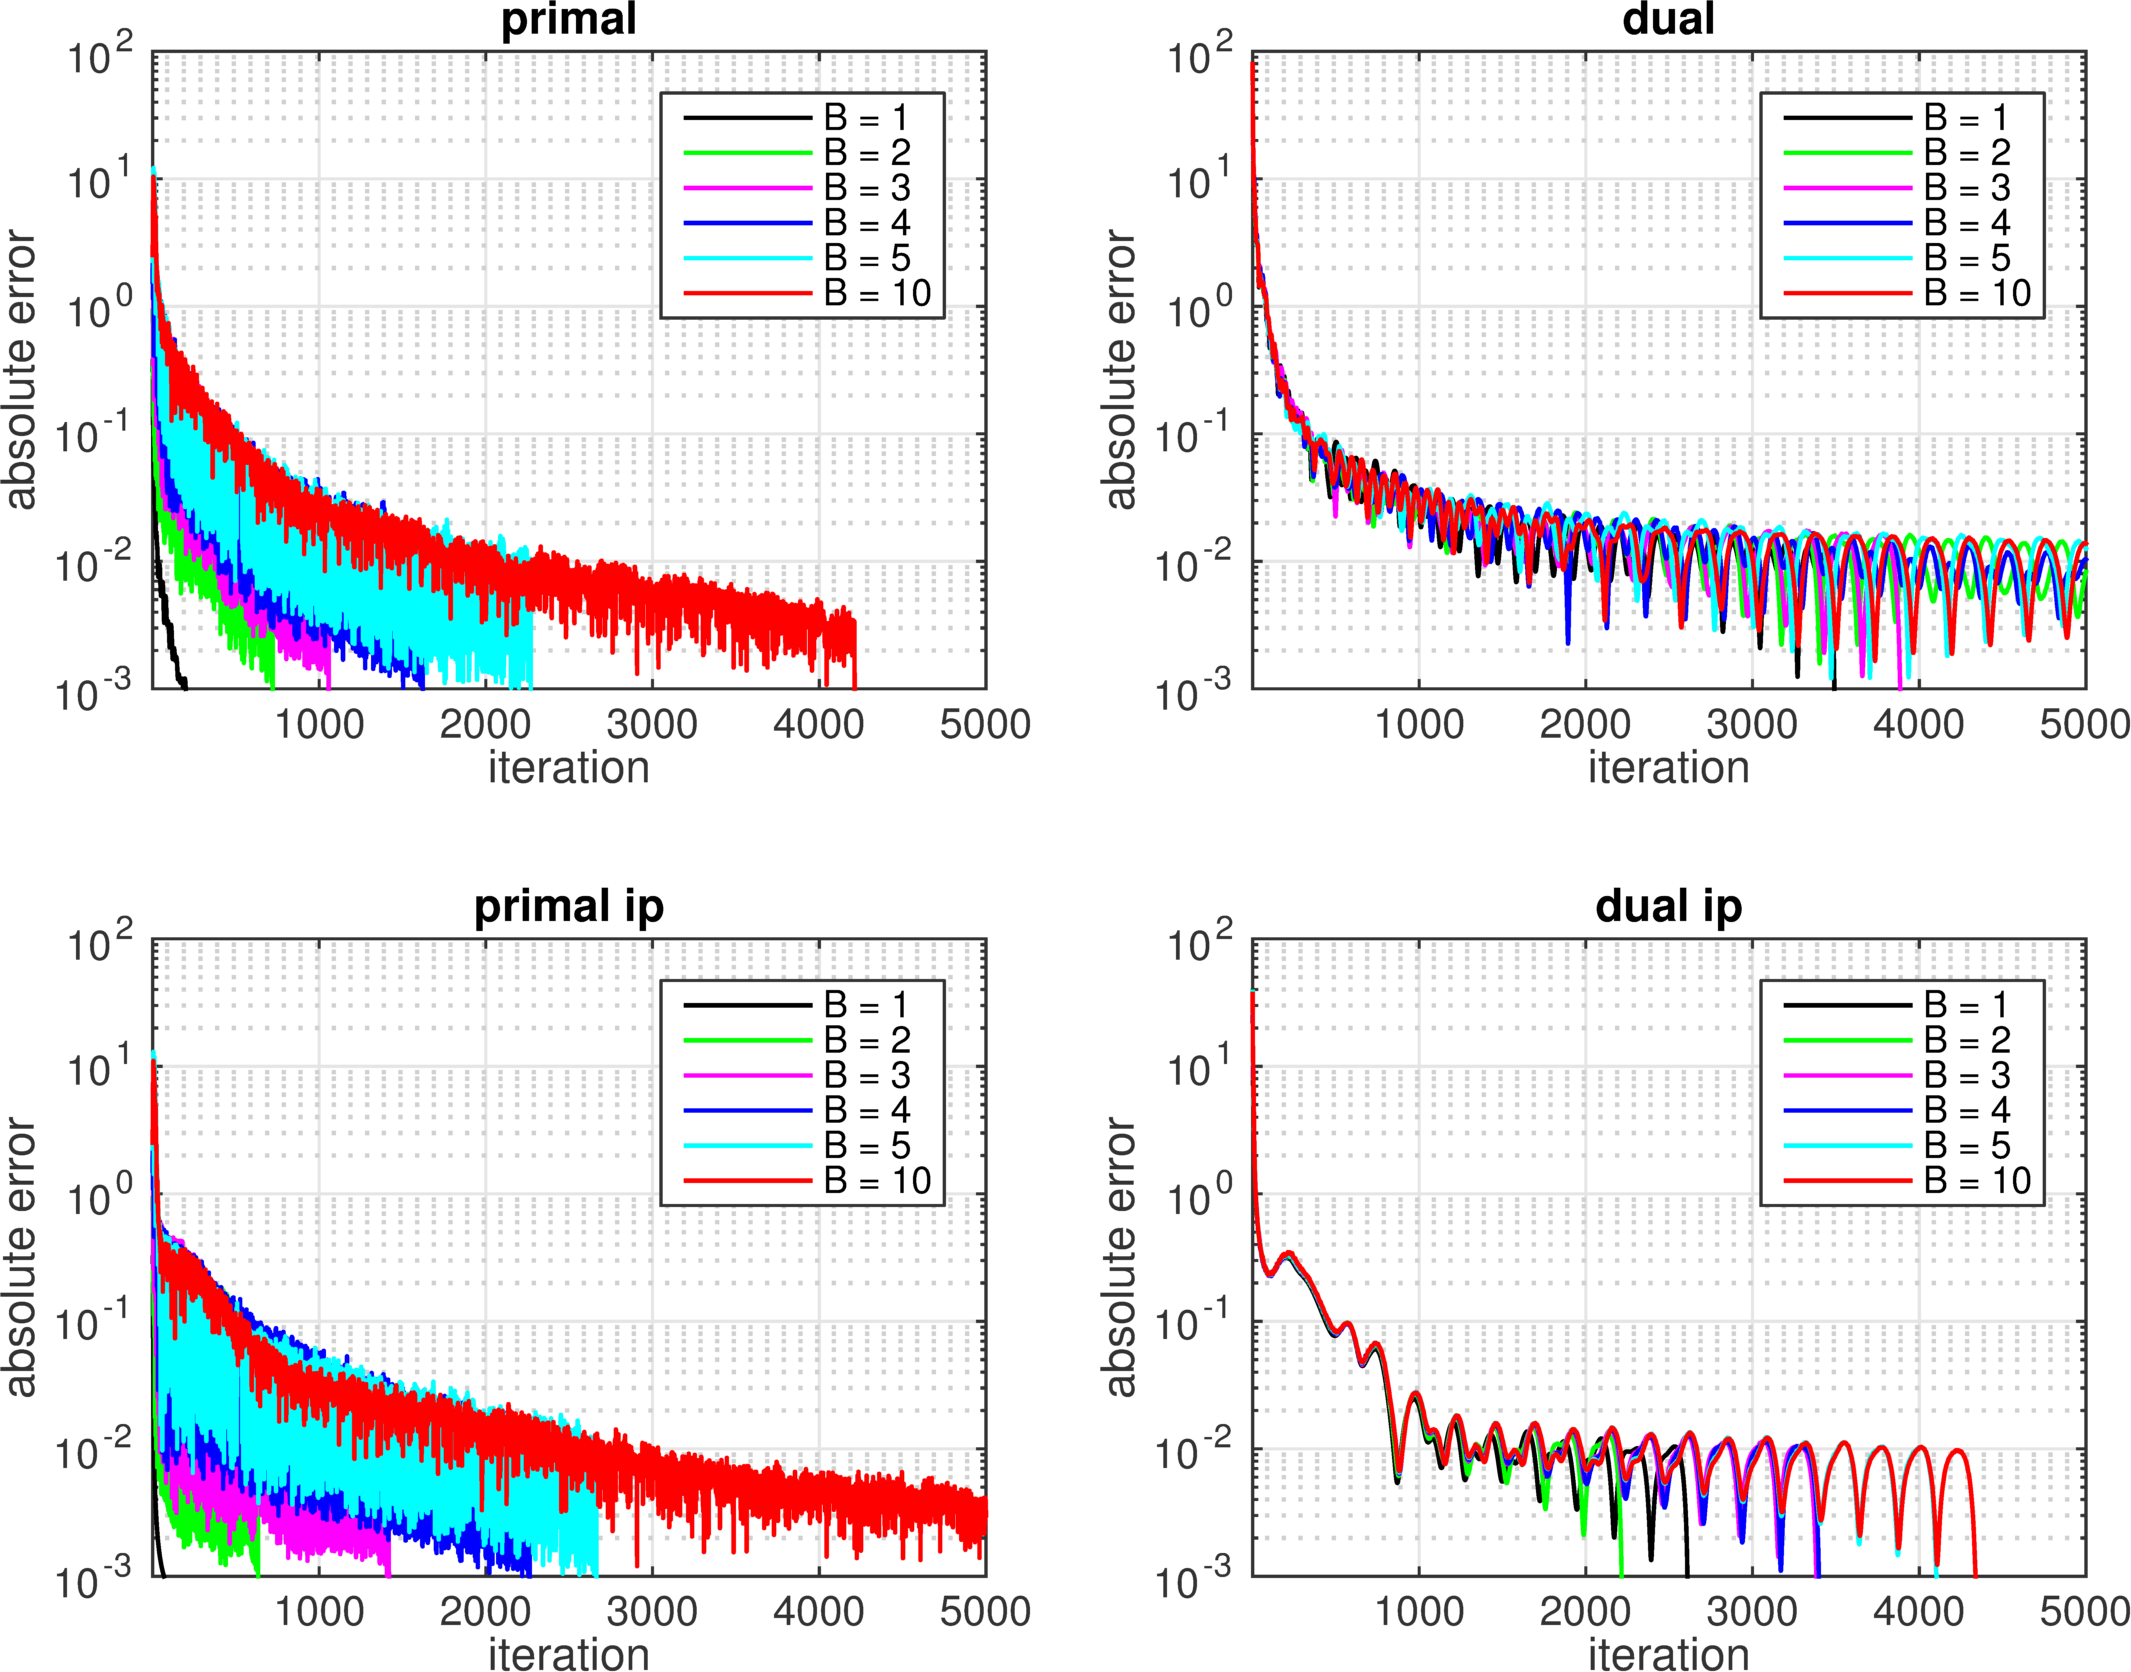
\includegraphics[width=\textwidth]{../figures/noprecond_rndperm.png}
	\caption{Results on a random LP problem of size $50 \times 300$. Only random permutation and no preconditioning.}
	\label{fig:nop_r}
\end{figure*}
\newpage
\subsection*{Block-splitting with Preconditioning (No Random Permutation)}
In this set of experiments, we applied preconditioning to each problem and used sequential block updates (no random permutation). The results are shown in Figure \ref{fig:p_nor}. Note that the number of blocks has no effect on the number of iterations required for either dual algorithm. This verifies our claim at the end of Section 3 that preconditioning applied to the dual causes $\mathbf{y}$ to be separable. Interestingly, the number of blocks has very little effect on the number of iterations for the primal. 

These results suggest that one should prefer to use the maximum number of blocks possible ($n$ for the primal and $m$ for the dual) when using preconditioning. In this case, the matrices that need to be inverted in the decision variable updates become scalars, so the updates can be computed rapidly.
\newline
\newline
\newline
\newline
\begin{figure*}[h]
	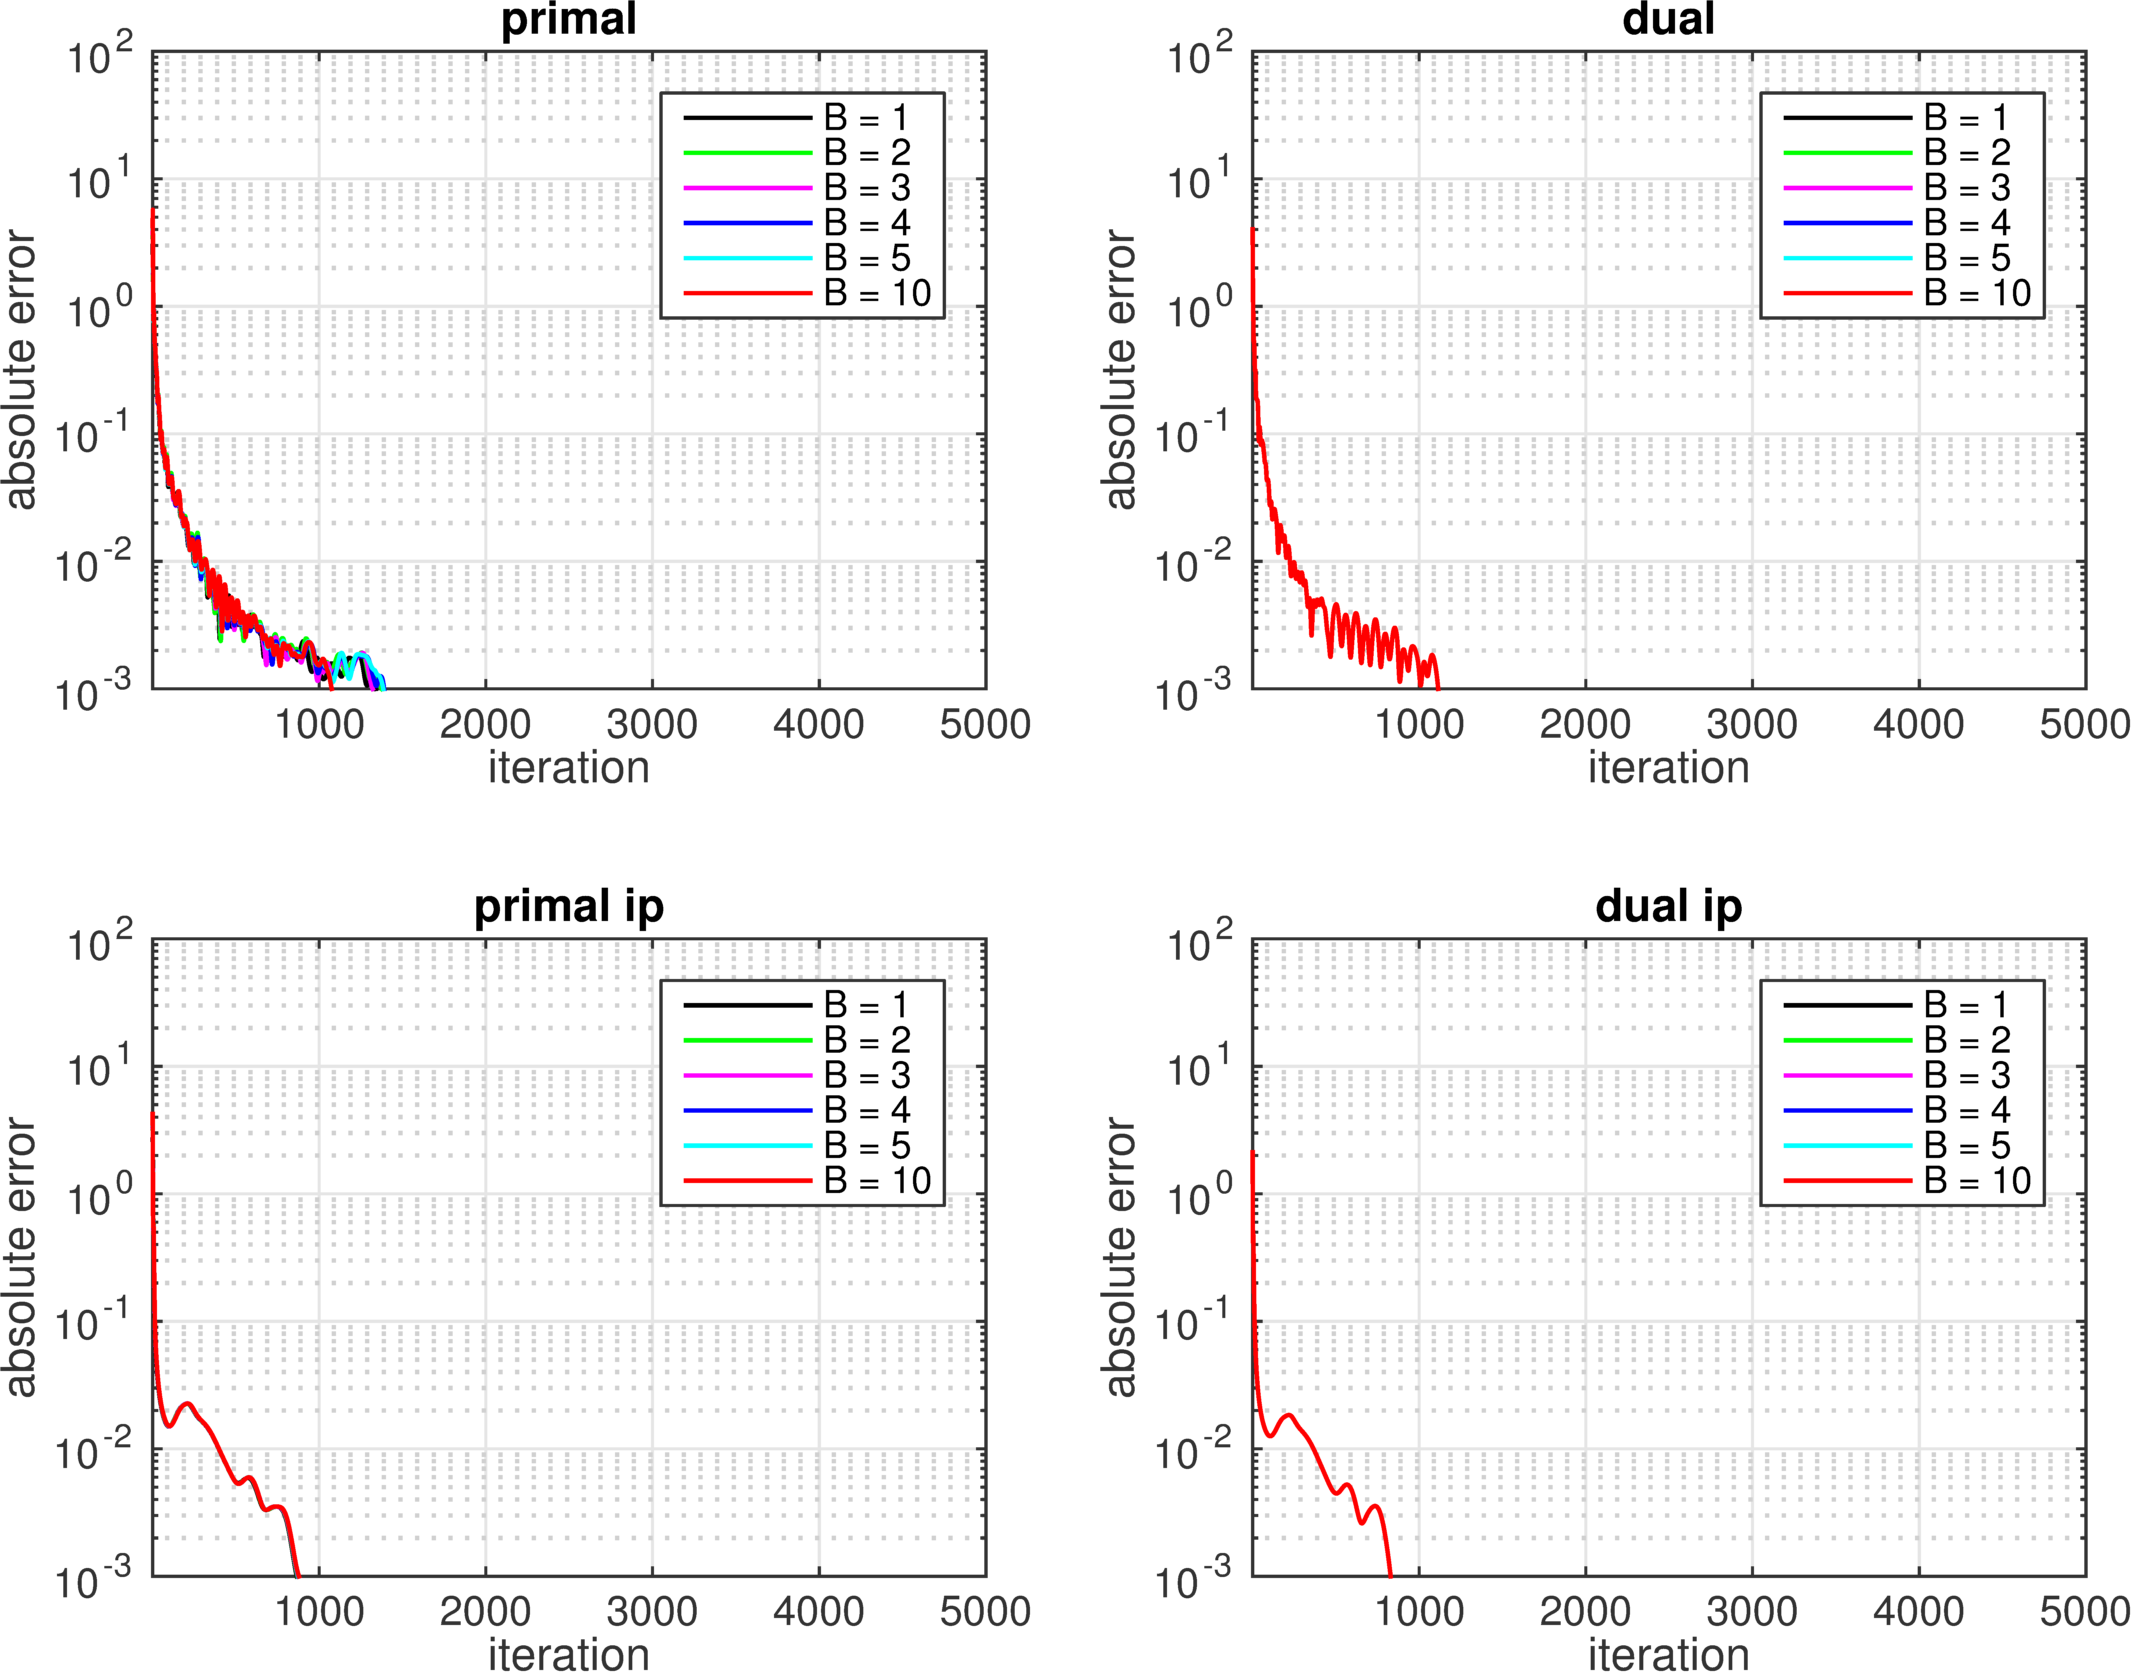
\includegraphics[width=\textwidth]{../figures/precond_norndperm.png}
	\caption{Results on a random LP problem of size $50 \times 300$. Only preconditioning and no random permutation.}
	\label{fig:p_nor}
\end{figure*}

\newpage
\subsection*{Analysis of Non-Converging Primal}
{\color{red} TODO: consider filling this out.}
In Figure \ref{fig:nop_nor}, we observed that the absolute error oscillates for \


\subsection*{Structured Problems}
In this set of experiments, we evaluated the performance of each ADMM algorithm when the matrix $A$ is composed of block structures. Figure \ref{fig:struct_prob} visualizes $A$ as a heatmap. This type of matrix structure is common in practice. Often, groups of related constraints only involve a subset of the decision variables, resulting in the "staircase" block structure in Figure \ref{fig:struct_prob}. Furthermore, there are often "coupling" constraints involving many decision variables, which is reflected in the last 10 constraints of $A$. It is natural to study whether performing block splitting along $A$'s block structures will improve the performance of ADMM. Note that $m=100$, $n=200$ for this set of experiments. 

\begin{figure*}[h]
	\centering
	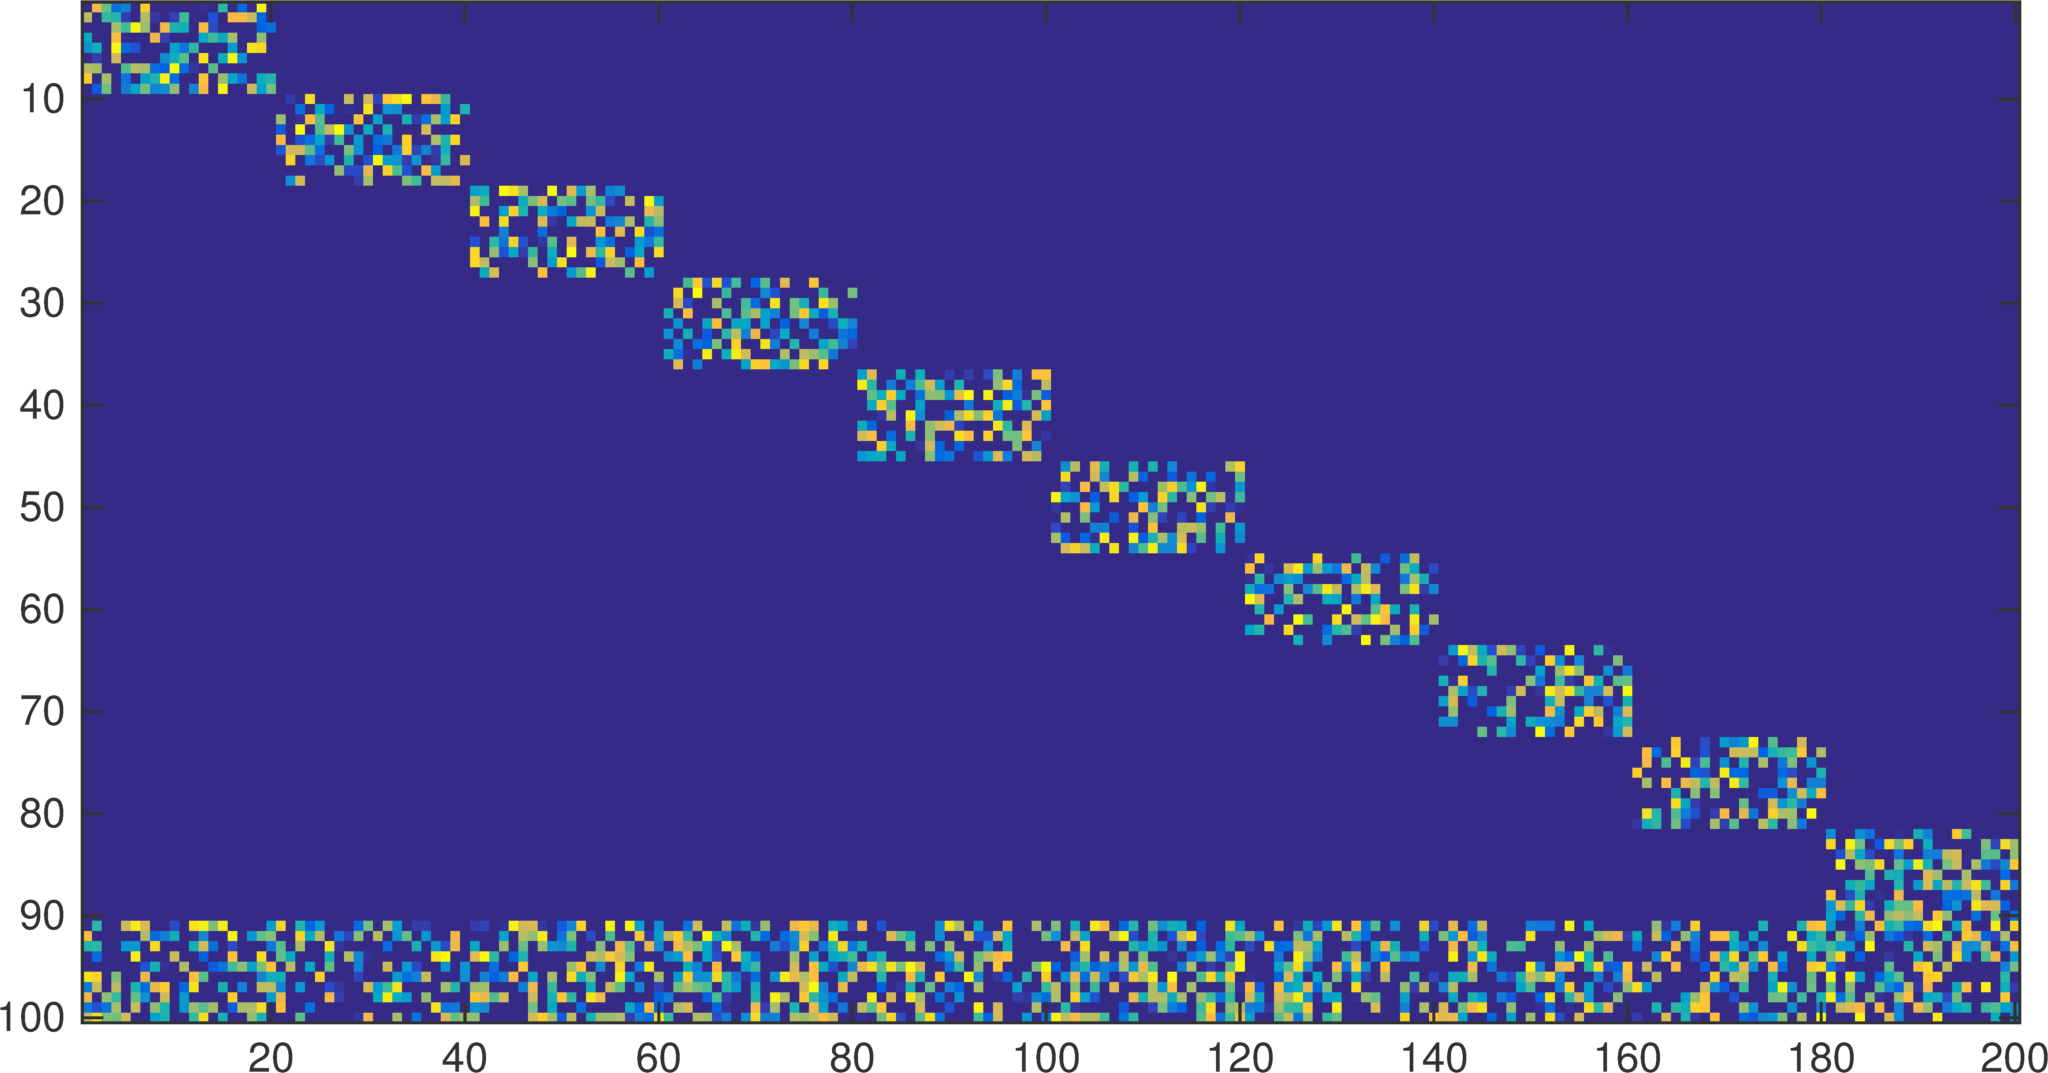
\includegraphics[width=0.8\textwidth]{../figures/struct_prob.png}
	\caption{Heatmap of Structured Matrix}
	\label{fig:struct_prob}
\end{figure*}

We re-ran each of the previous experiments on primal ADMM using the structured matrix $A$. Instead of performing arbitrary block splitting, we set $B=10$ and split the matrix $A$ along its block structures. The results of each experiment are shown in Figures \ref{fig:struct_nop_nor}-\ref{fig:struct_p_nor}.

In Figure \ref{fig:struct_nop_nor}, the problem diverges when applying block splitting for both the primal and the interior point primal formulations. This issue is not necessarily specific to structured matrices. We've observed that ADMM with block splitting (for $B>2$ will either fail to converge to the proper solution as in Figure \ref{fig:nop_nor} or diverge as in Figure \ref{fig:struct_nop_nor}. 


As in the non-structured case, we can resolve this issue by randomly permuting the block update order or applying preconditioning. The results for each approach are shown in Figures \ref{fig:struct_nop_r} and \ref{fig:struct_p_nor}. In both cases, the problem converges in approximately the same number of iterations as the single block case. The results are particularly striking for the preconditioning approach. These results suggest that performing optimal block splitting along a structured matrix may improve the performance of ADMM. In our future work, we plan to study whether this holds true in general for structured matrices.

\newpage
\begin{figure*}[ht!]
	\centering
	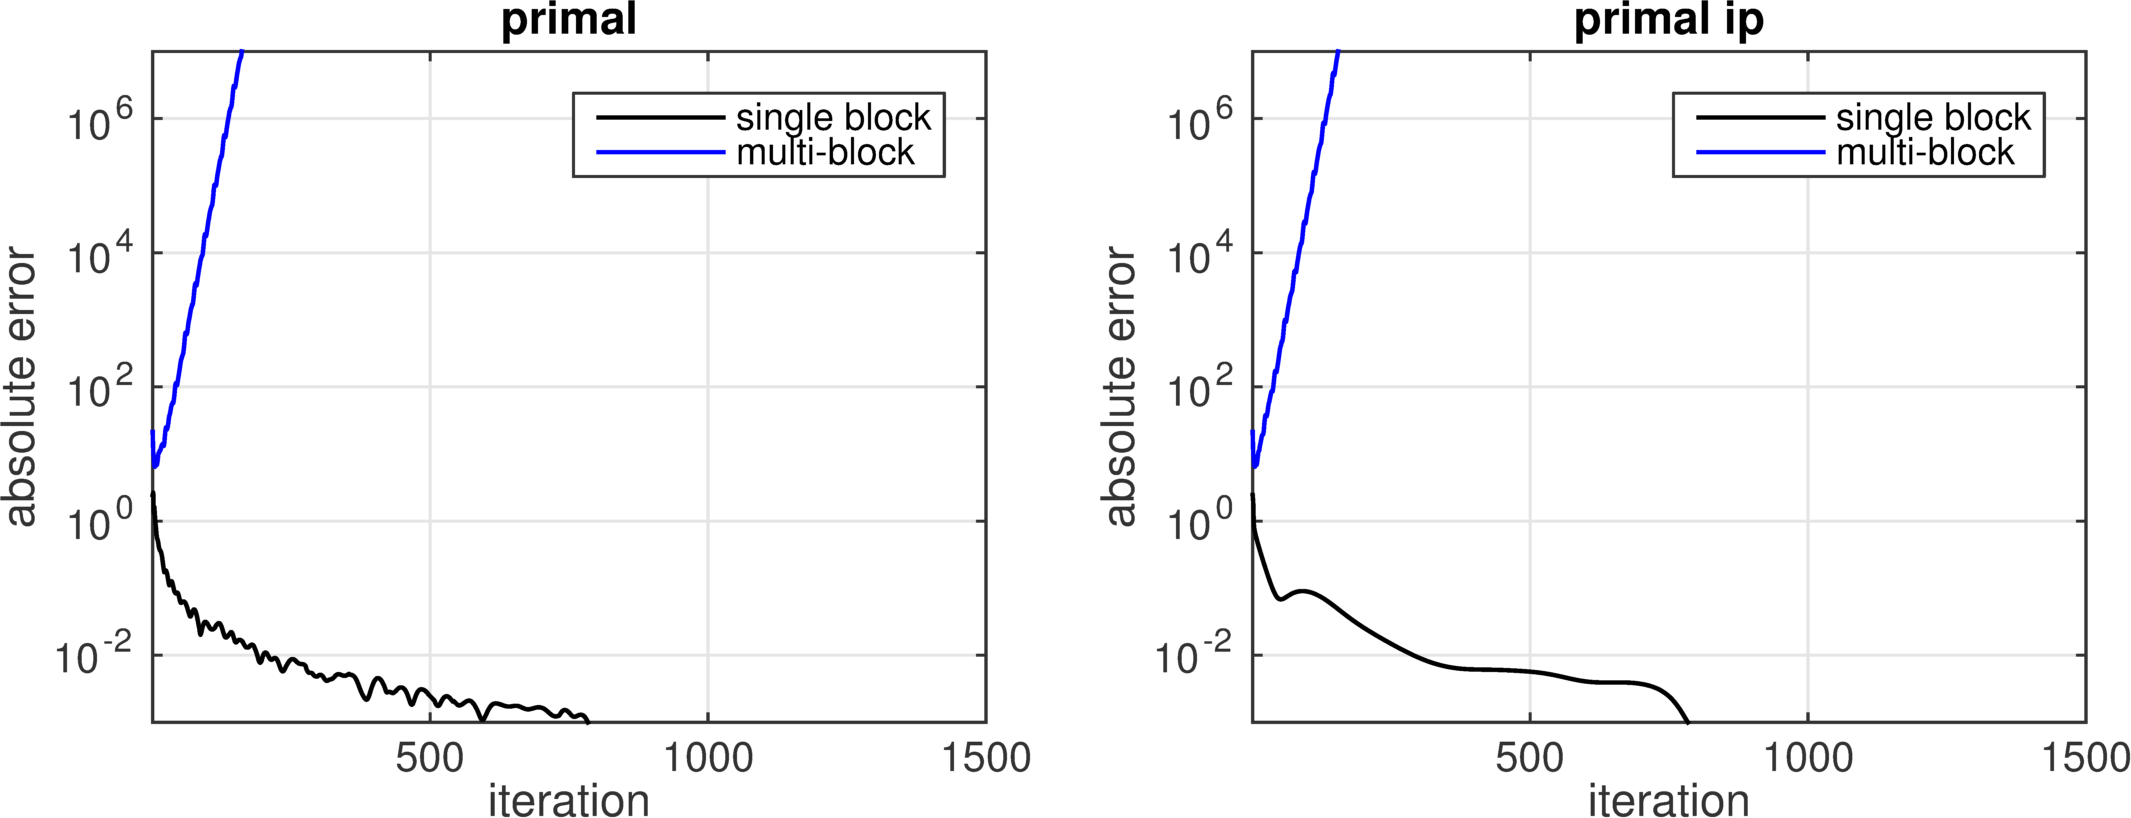
\includegraphics[width=0.9\textwidth]{../figures/struct_noprecond_norndperm.png}
	\caption{Structured problem. No preconditioning and no random permutation.}
	\label{fig:struct_nop_nor}
\end{figure*}
\begin{figure*}[ht!]
	\centering
	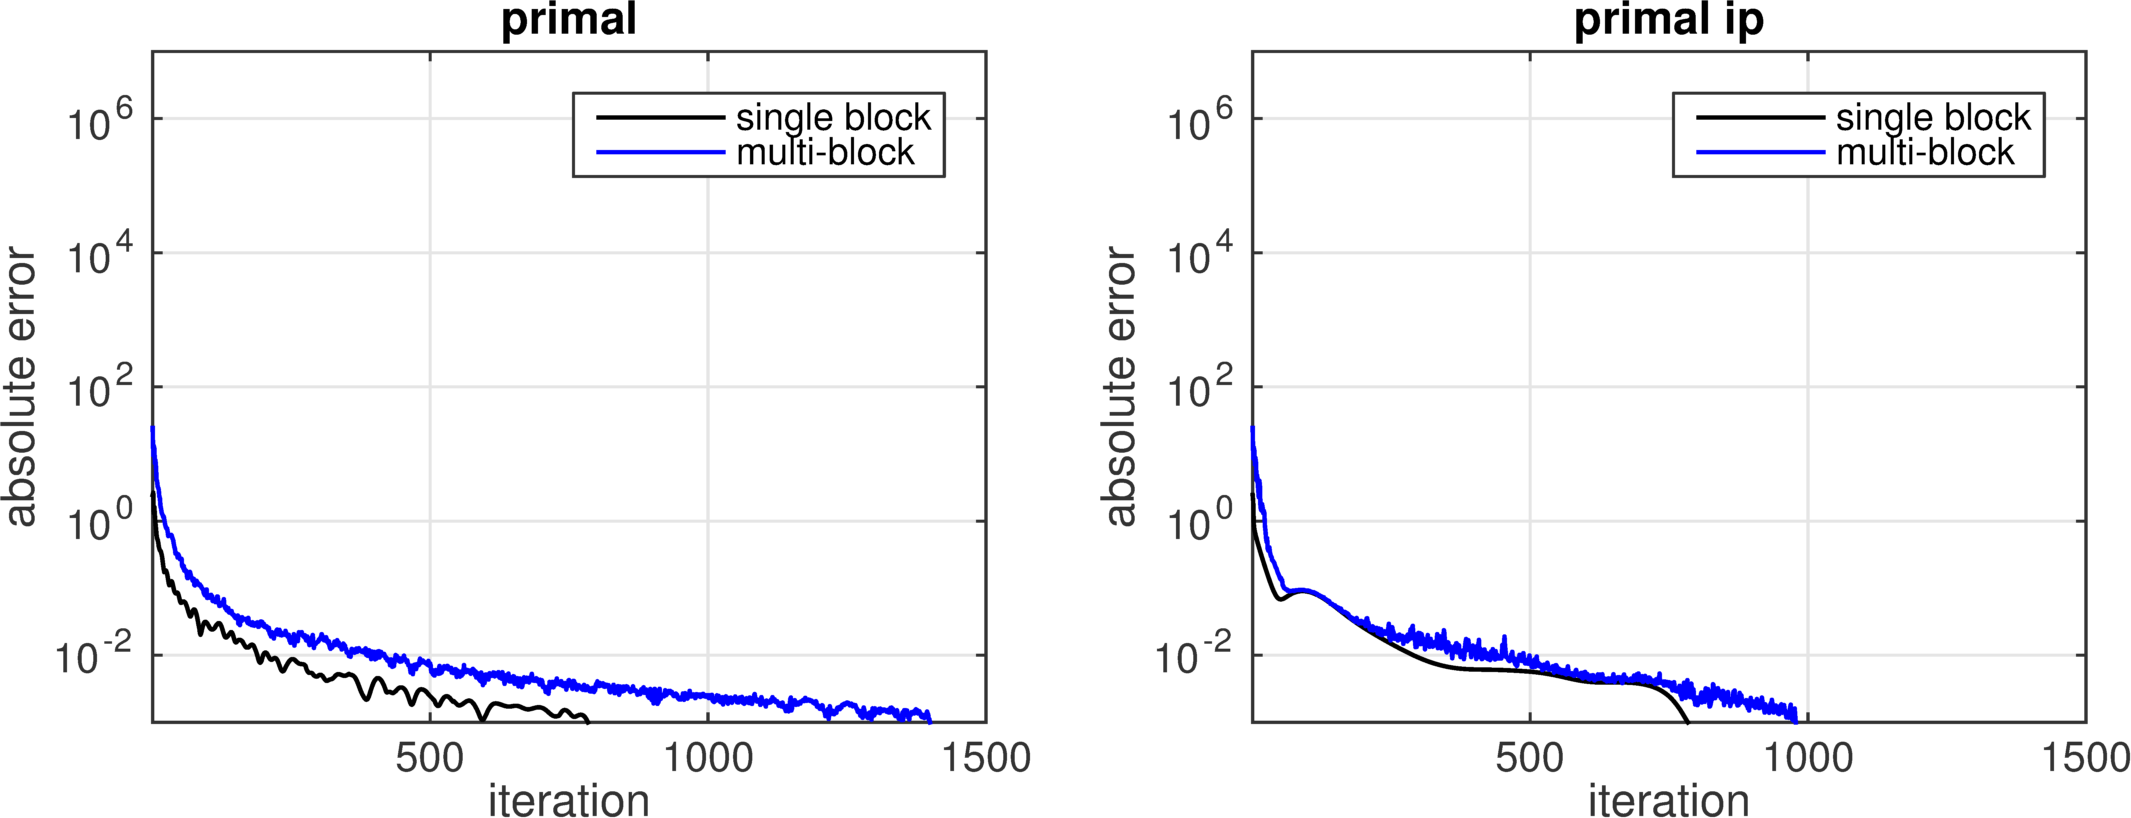
\includegraphics[width=0.9\textwidth]{../figures/struct_noprecond_rndperm.png}
	\caption{Structured problem. Only random permutation and no preconditioning.}
	\label{fig:struct_nop_r}
\end{figure*}
\begin{figure*}[ht!]
	\centering
	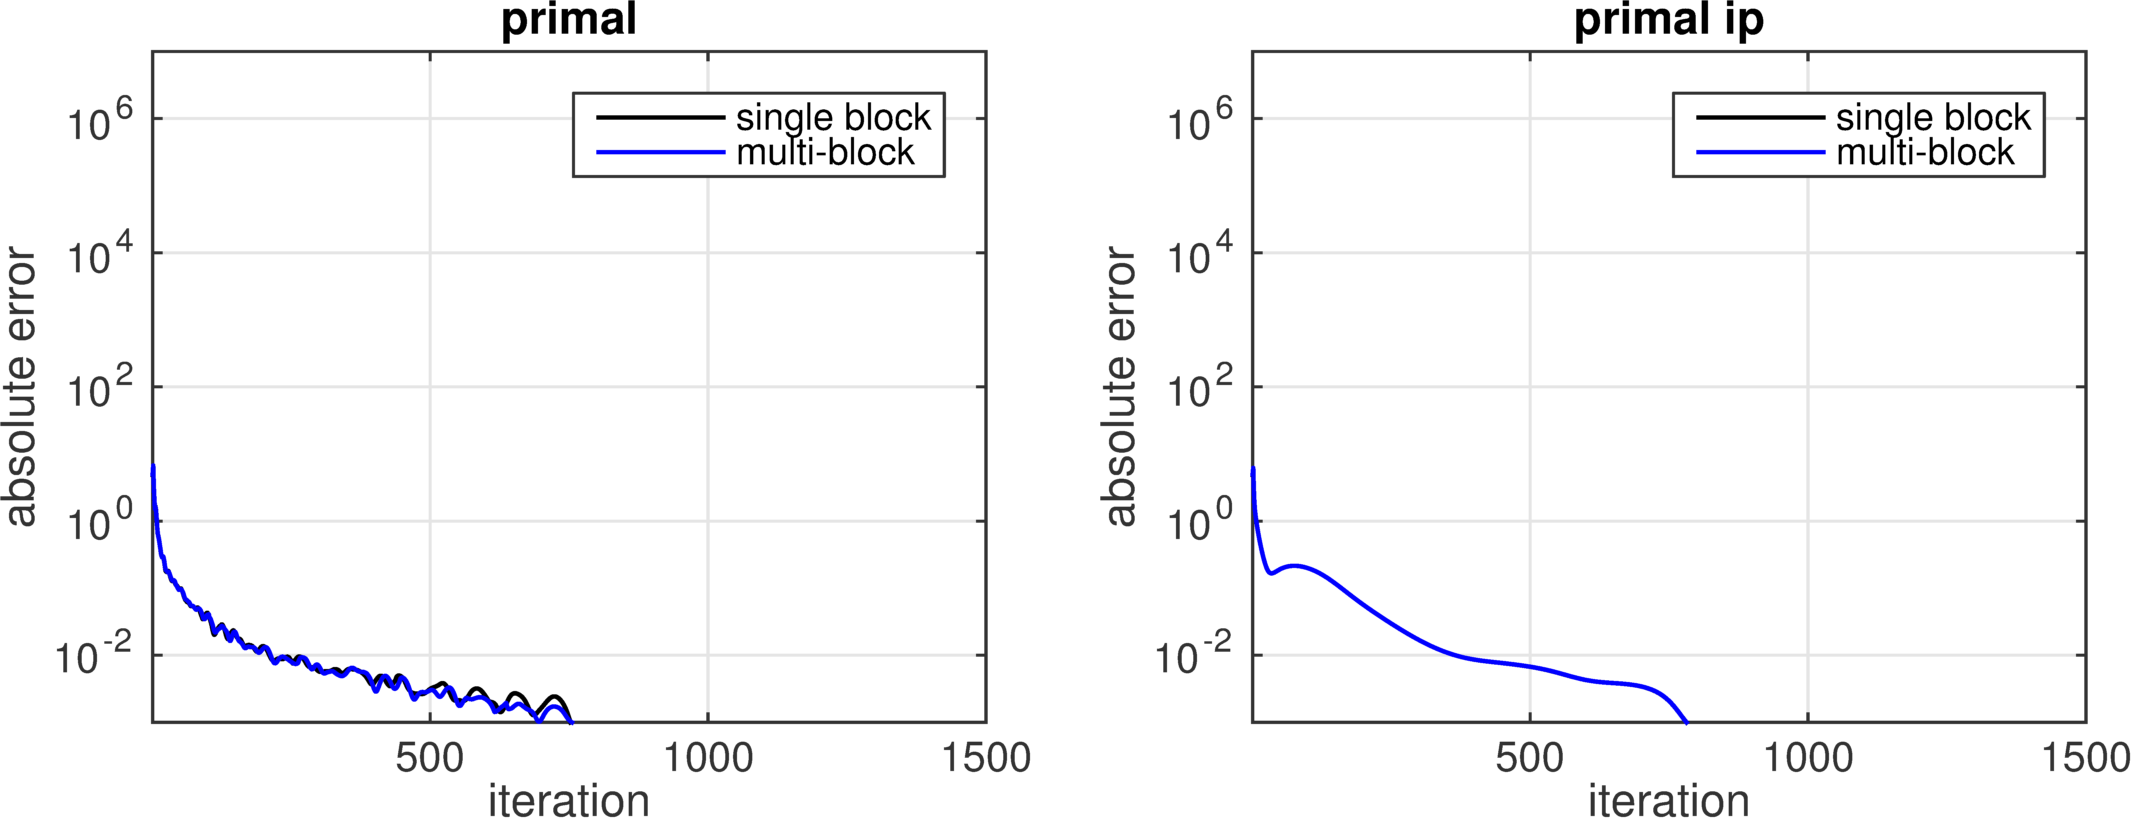
\includegraphics[width=0.9\textwidth]{../figures/struct_precond_norndperm.png}
	\caption{Structured problem. Only preconditioning and  no random permutation}
	\label{fig:struct_p_nor}
\end{figure*}


\newpage
\vspace{0.5in}
\section{Conclusions and Future Work}

We've evaluated the performance of several different versions of ADMM for linear programming problems. Our experiments show that one can split the problem into blocks without significantly increasing the number of iterations required to find an optimal solution. However, one must be sure to apply preconditioning to the problem or use a randomly permuted update order. Since block splitting allows one to avoid a large matrix inversion, our results suggest that these techniques may reduce the overall runtime of ADMM algorithms. We've also shown that block splitting seems especially well suited to problems with an inherent block structure, which commonly arise in practice.

In our future work, we intend to run similar experiments on more problems to verify that the results are robust. We also intend to test each approach on problems with various sizes. It will be interesting to see how each approach scales as problems grow large. In the future, we plan to compare the runtime (not just the number of iterations) of each algorithm. This will enable us to determine whether avoiding the large matrix inverse actually leads to a speedup. Finally, we intend to experiment with inverse-free preconditioning methods, such as Cholesky preconditioning, to avoid the matrix inversion involved in our current preconditioning approach.

\vspace{0.5in}
\section{Acknowledgements}

We'd like to thank Professor Yinyu Ye for his mentorship and guidance throughout the project. 

\newpage
\vspace{0.4in}
%\bibliographystyle{plain}
\bibliographystyle{ieeetr}
\end{document}
